\subsection{Bloklu atamaların tamamını saymak}

Bölüm~\ref{sec:v1-colt-park}'taki deney, Spector etiket karıştırmasına
tasarım bakımından karşı örnektir. Aşağıdaki kod yayımlanan veriden
hazırlanan 12 satırlık tabloyu kullanır. Diğer rejimler sabitken her
blokta dört parselden ikisi seçilir; bütün blokların seçimleri birlikte
ele alınır. Tek blokta döngü çalıştırıp çıkan $p$ değerlerinin ortalamasını
almak aynı test değildir.

\begin{lstlisting}[style=prismPythonApp]
from itertools import combinations, product
import numpy as np
import pandas as pd

veri = pd.read_csv(
    "companion/vakalar/v1-colt-park/comparison.csv")
bloklar = ["ONE", "TWO", "THREE"]
sayim = pd.crosstab(veri.block, veri.treatment)
assert veri.shape == (12, 4)
assert set(sayim.index) == set(bloklar)
assert set(sayim.columns) == {"FYM", "No Fertilizer"}
assert sayim.eq(2).all().all()
assert not veri.isna().any().any()
assert veri.source_row.is_unique
secenekler, gozlenenler = [], []
for blok in bloklar:
    alt = veri.loc[veri.block == blok]
    degerler = alt.dry_matter_g_m2.to_numpy()
    fym = alt.treatment.eq("FYM").to_numpy()
    gozlenenler.append(
        degerler[fym].mean()-degerler[~fym].mean())
    farklar = []
    for secim in combinations(range(4), 2):
        etiket = np.zeros(4, dtype=bool)
        etiket[list(secim)] = True
        farklar.append(degerler[etiket].mean()
                       - degerler[~etiket].mean())
    secenekler.append(farklar)
gozlenen = np.mean(gozlenenler)
dagilim = np.array([np.mean(secim)
                   for secim in product(*secenekler)])
uc = np.count_nonzero(
    np.abs(dagilim) >= abs(gozlenen)-1e-10)
assert len(dagilim) == 216
print(gozlenen, uc, len(dagilim), uc/len(dagilim))
\end{lstlisting}

\textbf{Çıktı:} Yaklaşık 171,487510717; 2; 216; 0,009259259259.
Eşit derecede uç değerleri kayan nokta yuvarlaması nedeniyle dışlamamak
için $10^{-10}$ g/m$^2$ tolerans kullanılır. Tam sayımda gözlenen atama
zaten dağılımın içindedir. Tohum veya tekrar sayısı değiştirerek bu sonucu
iyileştirmek söz konusu değildir.

\begin{figure}[H]
\centering
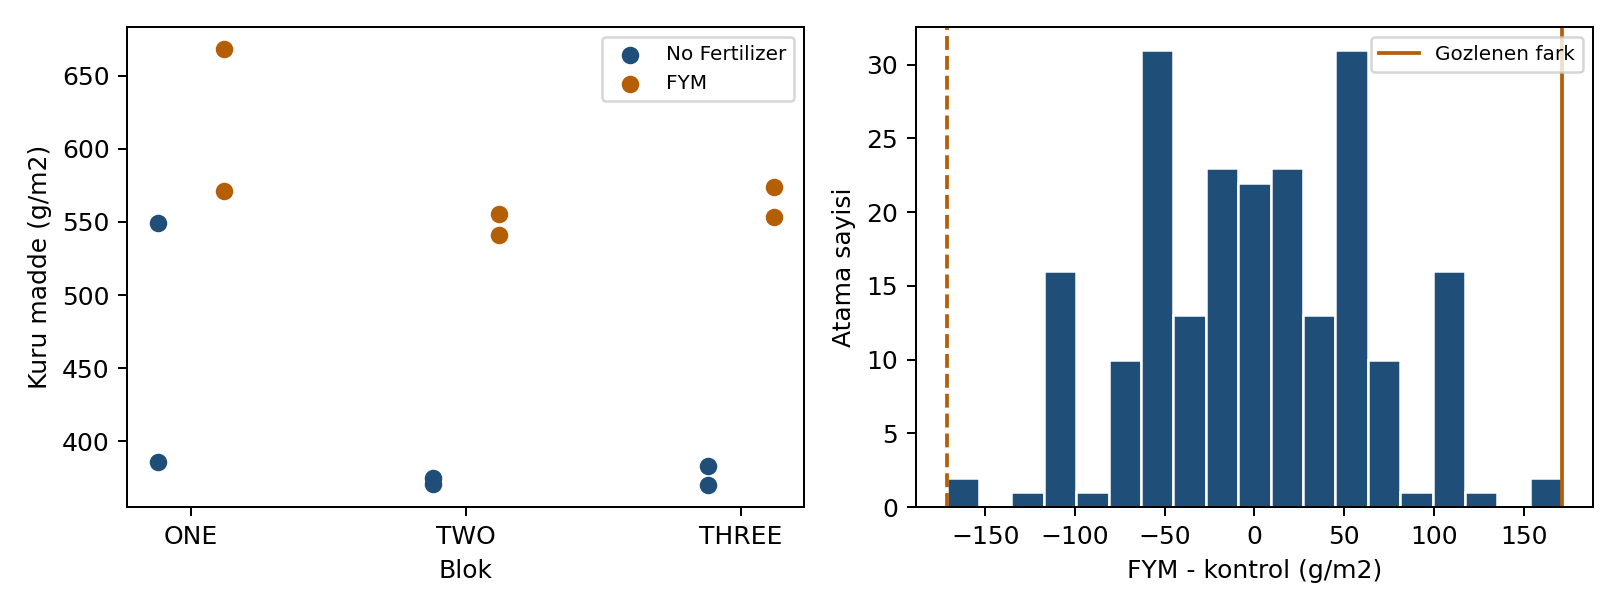
\includegraphics[width=\linewidth]{companion/vakalar/v1-colt-park/comparison.png}
\caption{Colt Park öğretim uyarlaması: solda 12 parselin yanıtı, sağda
216 koşullu atamanın fark dağılımı. Çizgiler gözlenen farkı ve negatifini
gösterir; histogram güven aralığı değildir.}
\label{fig:v1-colt-park}
\end{figure}

\textbf{Kontrol görevi.} Fark yönünü ters çevirin: tahminin işareti
değişmeli, mutlak değere dayalı iki yönlü $p$ aynı kalmalıdır.
Histogramın sınıf sayısını değiştirmenin tam sayım sonucunu neden
değiştirmediğini açıklayın; test grafiğin sütunlarından değil 216 değerden
hesaplanır.